% A projected entangled pair state on a four-by-four lattice.
%
% One tensor per site, joined to its neighbours by the bonds of the lattice and
% carrying one physical index of its own, out of the plane. The lattice is
% drawn turned by 45 degrees, so that it reads as a plane seen from above and
% every physical index can go straight down without crossing a bond. The
% boundary is open: a tensor at the edge simply has fewer bonds.
\documentclass[border=4pt]{standalone}
\usepackage{amsmath,amssymb}
\usepackage{tikz-tensors}
\input{notation}
\begin{document}
\begin{tikzpicture}
  \tngrid[legs]{P}{4}{4}{coef/$A$}
\end{tikzpicture}
\end{document}
